\documentclass[onecolumn]{article}
\usepackage{graphicx}
\usepackage{amsmath}
\usepackage{hyperref}
\usepackage{float}
\restylefloat{figure}

\begin{document}

\title{Analytical solution for a point source in a uniform ambient flow}

\author{Arjen Markus}

\maketitle

\section*{Introduction}
This note concerns the analytical solution of an idealised discharge situation. It is a
simplified model for localised sources of pollutants in an ambient flow, such occurs with
outfalls in sea or the discharge of production water at oil platforms. More specifically:
consider a uniform flow in an unbounded area. At the origin a point source of a pollutant is
located with a discharge small enough not to disturb the ambient flow.
To make things even simpler, we only consider a steady-state situation (see Fig.\ \ref{sketch_source}).

The area has a uniform depth \(H\) and the flow velocity is \(u\). The discharge has a concentration
\(C_s\) and a volume discharge of \(Q_s\), so that the mass rate is \(Q_s C_s\). Instead of the
concentration of a polluting substance, one may also consider thermal pollution, so that the
quantity of interest is the temperature increase. The (stationary) advection diffusion equation
describing the spreading of the pollutant is:

\begin{equation}
\label{AdvDiff}
\underline{u} \cdot \nabla C = D \nabla^2 C
\end{equation}

The boundary conditions that apply are:
\begin{itemize}
\item
At the origin there is a steady source of known strength, emitting the pollutant in a spherical-symmetric
fashion.
\item
Far from the source the concentration approaches zero, as the pollutant is mixed with ambient water.
\end{itemize}

The flow field, represented here by the vector \(\underline{u}\), may be thought to consist of two
components: the ambient flow \(u_0 \underline{e}_x\) and a radially outward component \(u_r \underline{e}_r\).
As long as the radial component is much less intense than the ambient flow one might consider the
total flow to be a superposition of these two, idealised, flows. In much of the remainder of this note,
however, we will assume that the radial component is negligible, as this makes the analytical solution
much simpler, while preserving most of the physics.

To analyse the problem we distinguish three regimes: the "overall" regime, a far-field regime where the
pollutant is distributed uniformly over the vertical and a near-field regime where the influence of the
bottom can be neglected.

\begin{figure}
\begin{center}
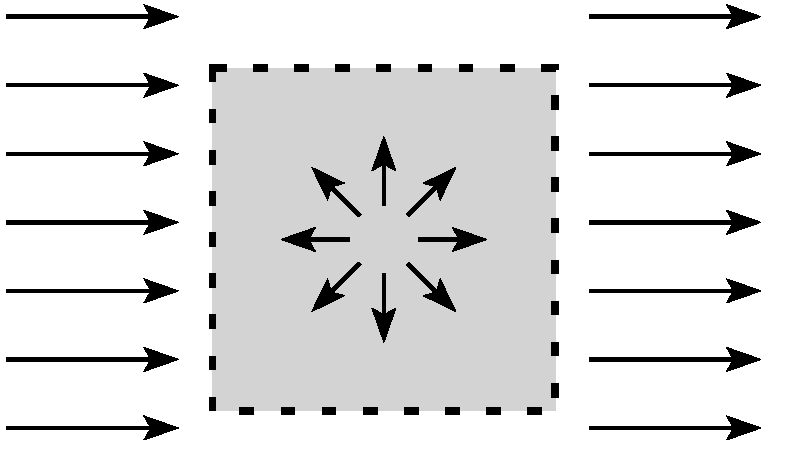
\includegraphics[width=60mm]{sketch_source.pdf}
\caption{Schematic representation of the flow field around a source. The grey square indicates
a control volume.}
\label{sketch_source}
\end{center}
\end{figure}

\section*{Overall regime}
Consider a box around the point source and assume that the pollutant is distributed uniformly over the
vertical, a "box approach" (see Fig.\ \ref{sketch_source}). The concentration on the downstream side is
approximately \(C\) and it is assumed that this concentration is also present on the two sides parallel
to the flow. The concentration on the upstream side is approximately zero. The mass balance therefore reads:

\begin{equation}
B H (u_0 - u_r) \cdot 0 + B H (u_0 + u_r) \cdot C + 2 B H u_r \cdot C = Q_s C_s
\end{equation}

\noindent where \(u_r = Q_s/4BH\) is the radial velocity component due to the volume of water discharged
by the point source and \(B\) is the side of the box.

We can now estimate the "mean" concentration inside the box:

\begin{equation}
    C = \frac{Q_s C_s}{B H (u_0 + 3 u_r)}
\end{equation}

To give an impression of the order of magnitude of this mean concentration:
\begin{itemize}
\item
Take the side of the box as \(10~m\), the depth as \(2~m\).
\item
The ambient flow velocity is \(0.2~m\).
\item
The discharge rate is \(0.2~m^3/s\) and the concentration is \(50~mg/l\).
\item
For the further analysis we need an estimate of the diffusion or dispersion coefficient as well. A practical
estimate is:
\begin{equation}
    D = \frac{1}{6} u_* H = \frac{1}{6} \frac{g^{1/2} u_0 H}{Ch}
\end{equation}
\noindent where \(Ch\) is the Ch\'ezy coefficient, typically around \(60~m^{1/2}/s\). This gives a
diffusion coefficient of \(0.02~m/s^2\)
\end{itemize}

Then the mean concentration in the box is: \(0.2 \cdot 50 / (2 \cdot 10 \cdot (0.2 + 3 \cdot 0.0025) \approx 2.5~g/m^3\)

\section*{Far-field regime}
The box approach has the disadvantage that we need to choose an arbitrary box width to get to a
concentration estimate. A more convenient approach is the following: if there is no ambient flow, the
pollutant will be spread in a axisymmetric pattern if it is well-mixed over the vertical or in a spherical
symmetric pattern if it is far away from the bottom. We can transform Eq.\ \ref{AdvDiff} so that the
resulting equation contains no advective term anymore:

\begin{equation}
C = e^{kx} \Gamma
\end{equation}

\noindent and Eq.\ \ref{AdvDiff} becomes:

\begin{equation}
k u_0 e^{kx} \Gamma + u_0 e^{kx} \frac{\partial \Gamma}{\partial x} = D \bigl ( k^2 e^{kx} \Gamma + 2 k e^{kx} \frac{\partial \Gamma}{\partial x} + e^{kx} \bigl ( \frac{\partial^2 \Gamma}{\partial x^2} + \frac{\partial^2 \Gamma}{\partial y^2} \bigr ) \bigr )
\end{equation}

Choosing the parameter \(k\) equal to \(u_0/2D\) means the first-order derivative terms cancel, yielding the
equation (after substituting \(k\) and dividing by \(\exp(kx)\)):

\begin{equation}
\label{Diff}
D \bigl ( \frac{\partial^2 \Gamma}{\partial x^2} + \frac{\partial^2 \Gamma}{\partial y^2} \bigr ) - k^2 \Gamma = 0
\end{equation}

This equation, essentially a reaction-diffusion equation with a first-order decay term,
allows both axisymmetric and spherical symmetric solutions in the form of modified
Bessel functions and modified spherical Bessel functions. The first case represents the far-field
approximation and the second the near-field.

The axisymmetric version of Eq.\ \ref{Diff} is:

\begin{equation}
\frac{1}{r}\frac{d}{dr} \bigl ( r \frac{d \Gamma}{dr} \bigr ) - k^2 \Gamma = 0
\end{equation}

We seek a solution that remains bound if \(r \rightarrow \infty\). This turns out to be a multiple of
the modified Bessel function of the second kind, \(K_0\), as the modified Bessel function of the first kind, \(I_0\),
increases as \(r \rightarrow \infty\). All we need to do now is to find the multiplication factor.
Since we know how much the point source discharges, we can equate that to the (diffusive) transport
around the point source (the factor \(\exp(kx)\) approaches 1 in the limit \(r \rightarrow 0\)):

\begin{equation}
- \int_0^{2 \pi} r H D \frac{d \Gamma}{d r} d \phi = - \int_0^{2 \pi} \gamma r H D \frac{d K(kr)}{d r} d \phi = Q_s C_s
\end{equation}

Using the asymptotic relation \(K(x) \rightarrow -\ln x\) for \(x \rightarrow 0\) we can approximate this
as follows:

\begin{equation}
  2 \pi \gamma D H = Q_s C_s \Rightarrow \gamma = \frac{Q_s C_s}{2 \pi D H} \approx 40~g/m^3
\end{equation}

For this regime to be valid, the pollutant must have spread uniformly over the vertical due to diffusion or
dispersion. The time scale associated with this mixing process is: \(T = H^2/D\). Due to the ambient flow
the distance over which the pollutant will have been transported is:

\begin{equation}
  L = u_0 T = u_0 H^2 / D
\end{equation}

With the above numerical values for the various quantities, this gives a length scale of \(40~m\).


\section*{Near-field regime}
In the near-field regime we assume both the bottom and the surface are "far" away, so that the solution to Eq.\ \ref{Diff} is
spherically symmetric:

\begin{equation}
\frac{1}{r^2}\frac{d}{dr} \bigl ( r^2 \frac{d \Gamma}{dr} \bigr ) - k^2 \Gamma = 0
\end{equation}

The general solution can be expressed in terms of the modified spherical Bessel functions of the first
and second kind, \(i_0\) and \(k_0\) respectively. As these are expressible in elementary functions,
the solution is quite simply (implementing the first boundary condition, so that the term with \(i_0\)
disappears):

\begin{equation}
\Gamma = \gamma k_0(kr) = \gamma \frac{e^{-kr}}{kr}
\end{equation}

The second boundary condition now is:

\begin{equation}
- \int_{-\pi/2}^{\pi/2} cos \theta \int_0^{2 \pi} r^2 D \frac{d \Gamma}{d r} d \phi d \theta = - \int_{-\pi/2}^{\pi/2} cos \theta \int_0^{2 \pi} \gamma r^2 D \frac{d k_0(kr)}{d r} d \phi d \theta = Q_s C_s
\end{equation}

This simplifies to:
\begin{equation}
4 \pi  \gamma r^2 D \bigl ( \frac{e^{-kr}}{r} + \frac{e^{-kr}}{kr^2} \bigr ) = Q_s C_s
\end{equation}

\noindent where \(r \rightarrow 0\).

If we take the numerical example again with a diffusion coefficient of \(0.02~m^2/s\):
\begin{equation}
\gamma = \frac{k Q_s C_s}{4 \pi D} = \frac{u_0 Q_s C_s}{8 \pi D^2} \approx 200~g/m^3
\end{equation}

The solution tends to infinity as the distance to the point source diminishes -- this is
the drawback of not including the radial component. However, a pragmatic argument could be that
the solution becomes valid only if the distance is large enough, say larger than the distance
where \(\Gamma\) becomes equal to \(C_s\). In the numerical example that distance is the root of
the equation:

\begin{equation}
\frac{e^{-kr}}{kr} = C_s / \gamma \Rightarrow kr \approx 1/2.5 \Rightarrow r = 1/2.5k \approx 8~cm
\end{equation}


\section*{Estimated concentration distribution}
By combining the two regimes we obtain an approximate concentration distribution for the entire
area. For the near-field regime the full solution is:
\begin{equation}
C = \frac{u_0 Q_s C_s}{8 \pi D^2} \frac{e^{kx - kr}}{kr}
\end{equation}

\noindent and for the far-field regime it is:
\begin{equation}
C = \frac{Q_s C_s}{2 \pi D H} e^{kx} K_0(kr)
\end{equation}

We can approximate these solutions on the x-axis as (\(r \equiv x\)) (see Fig.\ \ref{graph_xaxis}:
\begin{equation}
C = \frac{u_0 Q_s C_s}{8 \pi D^2 kx}
\end{equation}

For the far-field regime we take \(r \rightarrow \infty\), so that the modified Bessel function
can be approximated:
\begin{equation}
C = \frac{Q_s C_s}{2 \pi D H} e^{kx} K_0(kr) \approx \frac{Q_s C_s}{2 \pi D H} \sqrt{ \frac{2}{\pi k x}}
\end{equation}

As can be seen in the figure the two approximations give concentrations of the same order of magnitude.
For the region \(x \ll 40~m\) the near-field approximation should be used and for the region \(x \gg 40~m\)
the far-field approximation. In the intermediate region, the differences are fairly large. This
gives an impression of the pollutant concentration or the temperature increase downstream of a source.

\begin{figure}
\begin{center}
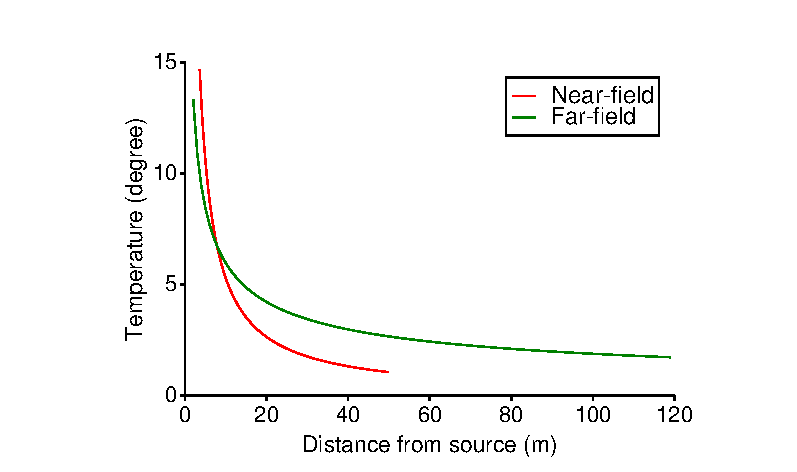
\includegraphics{graph_xaxis.pdf}
\caption{Concentration along the x-axis for the numerical example.}
\label{graph_xaxis}
\end{center}
\end{figure}

The profile along a line parallel to the y-axis can be approached by considering the region where \(y \ll x\):
\begin{equation}
r = \sqrt{x^2 + y^2} \approx |x| (1 + \frac{y^2}{2|x|})
\end{equation}
Then in the near-field regime:
\begin{equation}
C = \frac{u_0 Q_s C_s}{8 \pi D^2} kx e^{-ky^2/2x}
\end{equation}
\noindent and in the far-field regime:
\begin{equation}
C \approx \frac{Q_s C_s}{2 \pi D H} \sqrt{ \frac{2}{\pi k x}} e^{-ky^2/2x}
\end{equation}

So in both regimes the width of the plume is of the order \(2\sqrt{xD/u_0}\). Using the numerical example
again: at a distance of 1~km the plume reaches a width of 10~m, at a distance of 10~km it is 30~m wide,
whereas the concentration is in the order of 0.5 respectively 0.15~\(g/m^3\). Thus such a
plume remains fairly confined and this poses restrictions on the spatial resolution of numerical models.

\end{document}
